\documentclass[aspectratio=169]{beamer}
\usepackage{multicol}
\usepackage{qrcode}
\usepackage{datetime}
\usepackage{hyperref}
\usepackage{xcolor}
\usepackage{tikz}

\usetheme{Antibes}
\setbeamertemplate{footline}[frame number]{}

\newcommand{\makemycolor}[2]{%
    \pgfmathsetmacro{\hue}{(#1/100)^1.715*0.79}%
    \definecolor{myhsbcolor}{hsb}{\hue,1,1}%
    \textcolor{myhsbcolor}{#2}%
}

\hypersetup{
    colorlinks=true,
    linkcolor=blue,
    filecolor=magenta,      
    urlcolor=blue,
    pdftitle={Il Mining},
    pdfpagemode=FullScreen,
    }

\urlstyle{same}

\title{Il Mining} 
\author{Valerio Vaccaro}
\newdate{date}{04}{03}{2024}
\date{\displaydate{date}}
\logo{}

\begin{document}

\begin{frame}[plain,noframenumbering]
    \titlepage
    \begin{center}
        
\includegraphics[height=1cm]{logo.png}
    \end{center}
\end{frame}

\begin{frame}[noframenumbering]
    \tableofcontents
\end{frame}

\begin{frame}{Meme}
    \begin{center}
        
\includegraphics[height=5cm]{meme_3.png}
    \end{center}
    * entro la fine del corso capirete tutti i meme.
\end{frame}

\begin{frame}{Riassunto}
    \begin{itemize}
        \item Strutture dati blocco ed header
        \item Altezza e block id
        \item Merkle tree
        \item Blocco 0 e coinbase
        \item Testnet/signet/regtest
        \item ...
    \end{itemize}
\end{frame}

\section{Il Mining - L’economia di Bitcoin e la creazione di valuta}

\begin{frame}{Mining}
    \begin{alertblock}{da "Mastering Bitcoin"}
        "Lo scopo del mining non è la creazione di nuovi bitcoin. Questo è un sistema di incentivi. Il mining è il meccanismo con cui la
        sicurezza di bitcoin è decentralizzata."
    \end{alertblock}

    La scelta del nome mining non è particolarmente felice, il mining si occupa di:
    \begin{itemize}
        \item Gestire l'emergenza di un nuovo consenso senza autorità centrale
        \item Rendere costosa/impossibile la modifica delle storia di Bitcoin
        \item Consolidare le transazioni
        \item Creare nuova moneta
    \end{itemize}
\end{frame}

\begin{frame}{L'economia del miner}
    Costi:
    \begin{itemize}
        \item Corrente elettrica
        \item Hardware specializzato per il mining
        \item Gestione e manutenzione
    \end{itemize}

    Ricavi:
    \begin{itemize}
        \item Premio (attualmente 6,25 BTC)
        \item Somma delle fee pagate da tutte le transazioni incluse
    \end{itemize}

    I ricavi sono spendibili dopo 100 blocchi, se il blocco è considerato non-valido i ricavi non potranno essere mai spesi.
\end{frame}

\begin{frame}{L'economia di Bitcoin}
    Ogni 210.000 blocchi il premio si dimezza.
    \begin{center}
        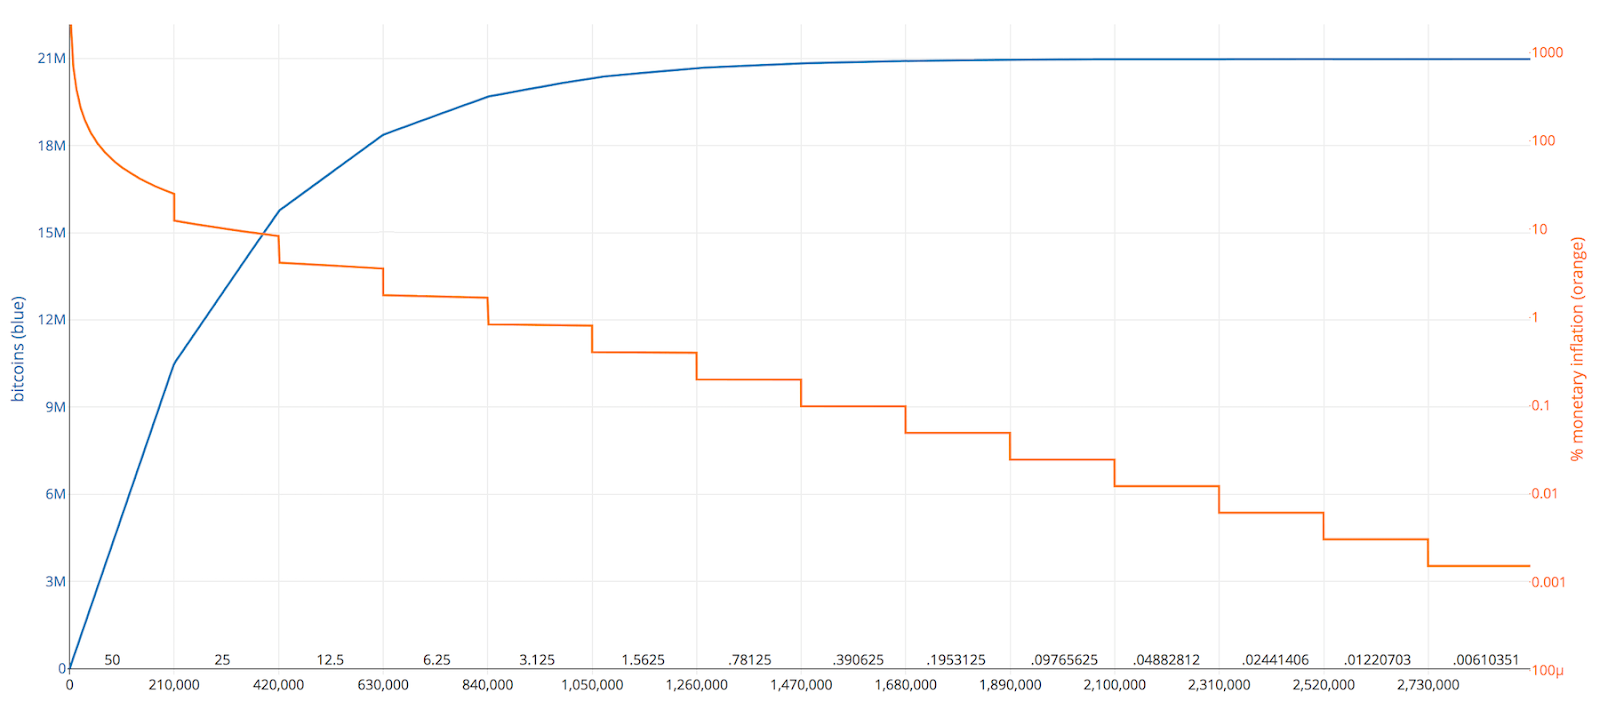
\includegraphics[height=5cm]{halving.png}
    \end{center}
    Nel 2140 (circa) saranno generati tutti i 21 milioni di Bitcoin.
\end{frame}

\begin{frame}{L'economia di Bitcoin}
    I Bitcoin sono in un numero finito.
    
    Perché?

    "L’emissione limitata e decrescente crea un approvvigionamento monetario fisso che resiste all’inflazione. A differenza di una moneta fiat, che può essere stampata in numeri infiniti da una banca centrale, il bitcoin non può mai essere gonfiato con la stampa"

    -- Mastering Bitcoin
\end{frame}

\section{Costruzione Block Header}

\begin{frame}{Costruzione del blocco}
    Per minare un nuovo blocco dobbiamo prima costruirlo.
    \begin{center}
        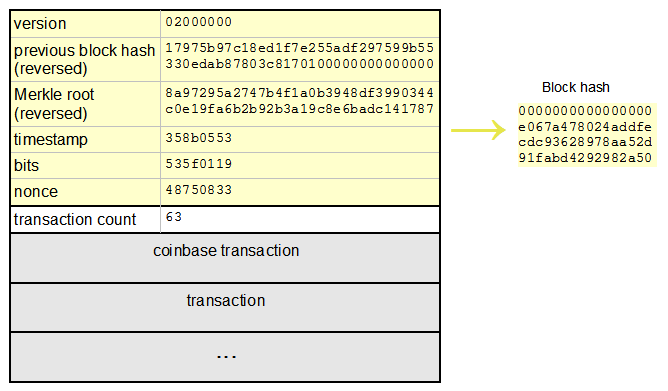
\includegraphics[height=5cm]{blocco_struct.png}
    \end{center}
\end{frame}

\begin{frame}{Selezione delle transazioni}
    Il primo step è cercare la lista delle transazioni che includeremo nel nuovo blocco.

    Validate le transazioni scegliamo il mix in modo da:
    \begin{itemize}
        \item Riempire lo spazio del blocco il più possibile
        \item Massimizzare la somma delle fee pagate da tutte le transazioni scelte
    \end{itemize}
    Che è una variate del "Problema dello zaino" e quindi NP-completo.
\end{frame}

\begin{frame}{Selezione delle transazioni}
    Poi dobbiamo aggiungere la coinbase che è una transazione speciale che ha le seguenti caratteristiche:
    \begin{itemize}
        \item Può avere zero fee
        \item Può non avere input (cioè generare nuova moneta)
        \item Può avere uno o più output la cui somma sia inferiore o uguale al premio più la somma delle fee pagate dalle transazioni
    \end{itemize}

    \begin{alertblock}{Fee}
        Le fee non sono in consenso quindi un blocco può contenere transazioni che non pagano fee, il miner normalmente scarterà queste transazioni. Probabilmente anche la mempool le scarterà per una protezione da attacchi DOS.
    \end{alertblock}
\end{frame}

\begin{frame}{Selezione delle transazioni}
    Spesso la coinbase al posto degli input ha dei dati (random o meno) che aiutano l'attività di mining (questo spazio è normalmente chiamato extra nonce).
    
    \begin{alertblock}{Extra Nonce}
        Visto che il campo Nonce dell'header è di dimensioni troppo piccole per il mining viene utilizzato anche il campo extra nonce per generare diversi template di transazione su cui effettuare il mining.
    \end{alertblock}
\end{frame}

\begin{frame}{Costruzione dell'header}
    \begin{center}
        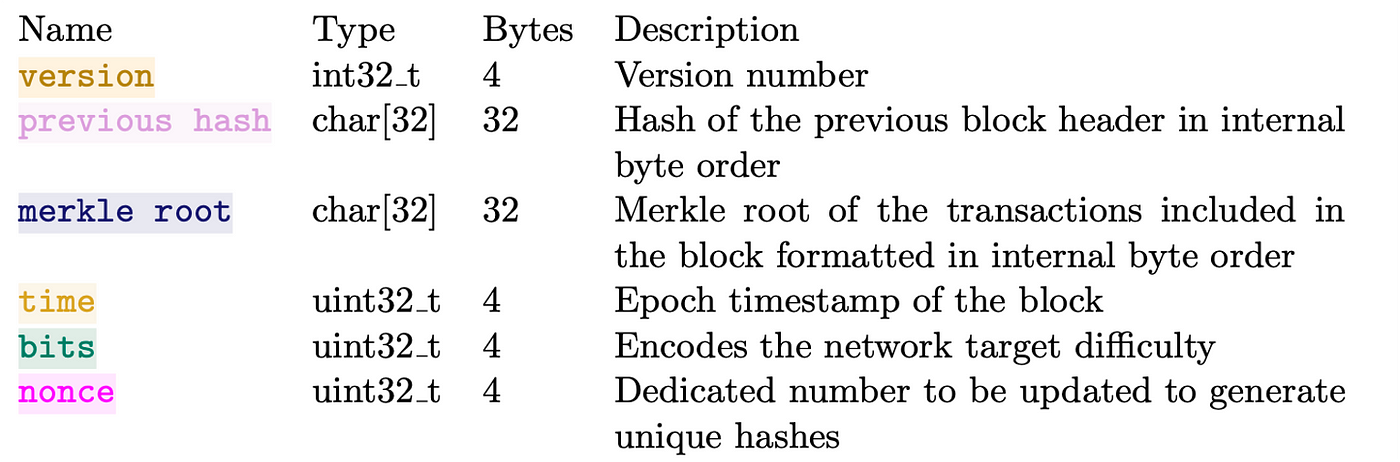
\includegraphics[height=5cm]{header_colorato.png}
    \end{center}
\end{frame}

\begin{frame}{Costruzione dell'header}
    \begin{itemize}
        \item Mettiamo la versione a 2
        \item Copiamo il block id del blocco precedente
        \item Calcoliamo il merkle tree di tutte le transazioni (coinbase compresa) e copiamo il merkle root
        \item Copiamo il timestamp dal nostro computer (assicuriamoci sia aggiornato)
        \item Copiamo il target (o ricalcoliamolo se necessario)
        \item Poniamo nonce a zero
    \end{itemize}
\end{frame}

\begin{frame}{Target}
    \begin{center}
        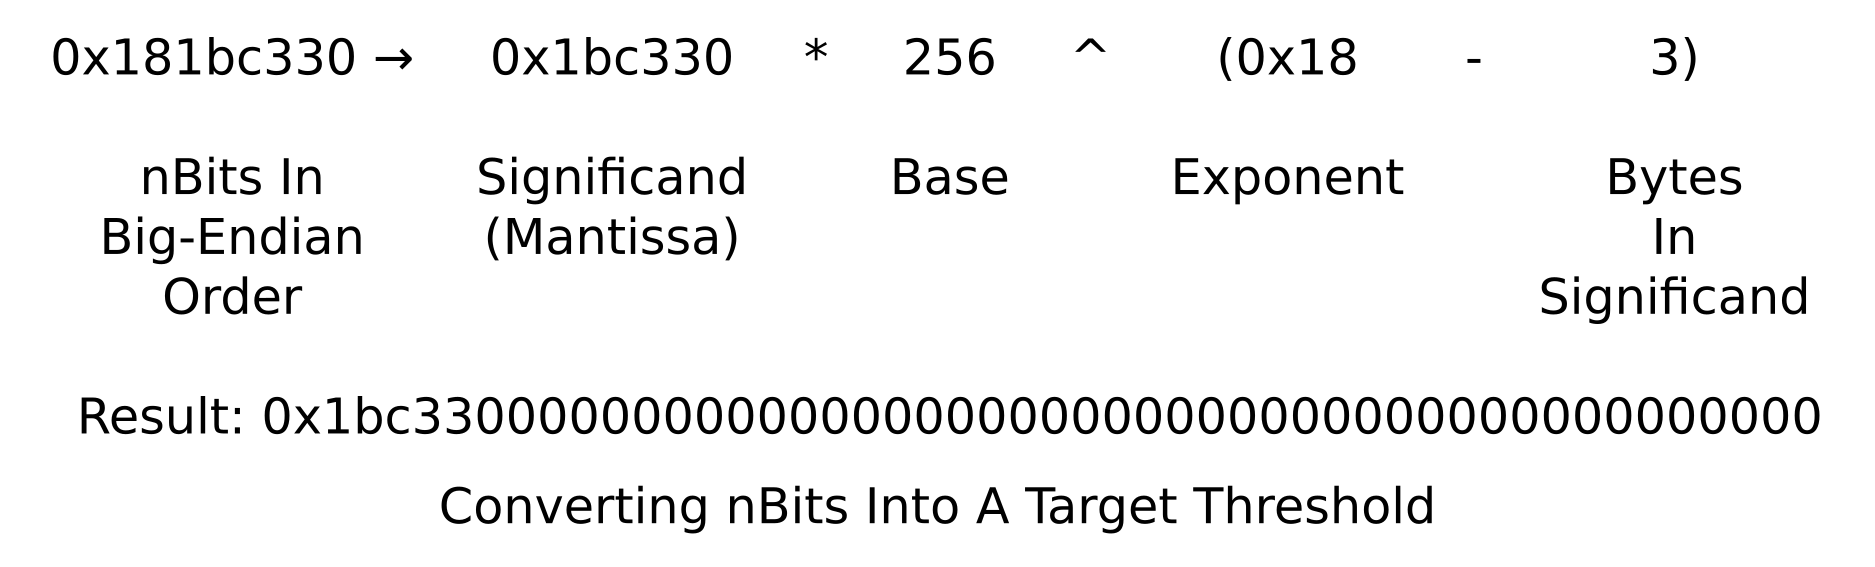
\includegraphics[height=4cm]{target.png}
    \end{center}
\end{frame}

\section{Mining del Blocco}

\begin{frame}{Mining}
    Occorre trovare un nonce (in generale un header) il cui hash sia minore del target (o più facile da ricordare con un certo numero di zeri).
    \begin{center}
        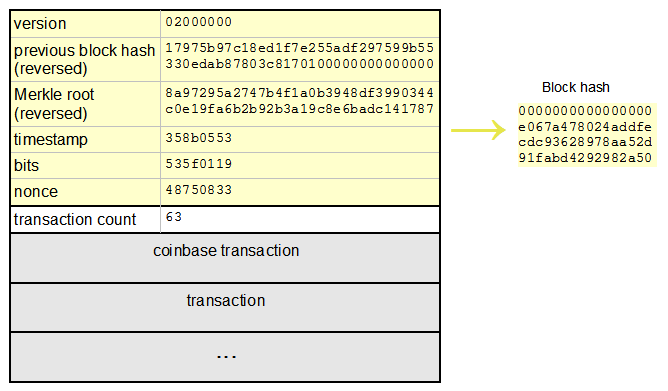
\includegraphics[height=5cm]{blocco_struct.png}
    \end{center}
\end{frame}

\begin{frame}{Ottimizzazione}
    L'header di un blocco è grande 80 byte, SHA256 lavora a blocchi di 64 byte.

    Il nonce si trova oltre i primi 64 byte quindi potremmo:
    \begin{itemize}
        \item Calcolare SHA256 dei primi 64 byte SENZA finalizzare e memorizzare il risultato come S
        \item Applicare ad S il nonce e finalizzare SHA256
        \item Ripetere il punto precedente per tutti i valori di nonce
    \end{itemize}

    Abbiamo velocizzato di parecchio il mining per Bitcoin.
\end{frame}

\begin{frame}{Solomining vs. pool}
    Fino ad ora abbiamo visto come fare minig in solitaria ovvero senza collaborare con altri (solomining).
    Se il nostro hashrate è basso potremmo dover aspettare anni per trovare la soluzione ad un blocco.
    
    Le pool nascono per aggregare il lavoro da più miner e fornire pagamenti a scadenze regolari (o al raggiungimento di un certo target).

    In cambio le pool si prendono una percentuale e forniscono dei servizi web con cui istruire il proprio miner.
\end{frame}

\begin{frame}{Evoluzione tecnologica del mining}
    \begin{center}
        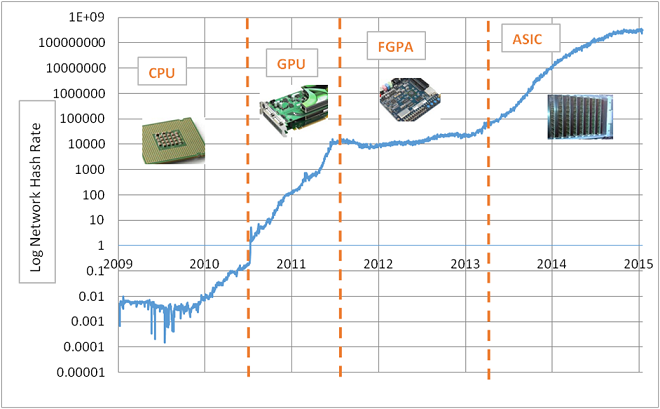
\includegraphics[height=5cm]{hashrate.png}
    \end{center}     

    Il mining ricerca:
    \begin{itemize}
        \item Energia a prezzo inferiore (di qualsiasi tipo)
        \item Nuove tecnologie che riescano ad effettuare mining ad un costo inferiore
    \end{itemize}
\end{frame}

\begin{frame}{Pausa}
    \begin{center}
        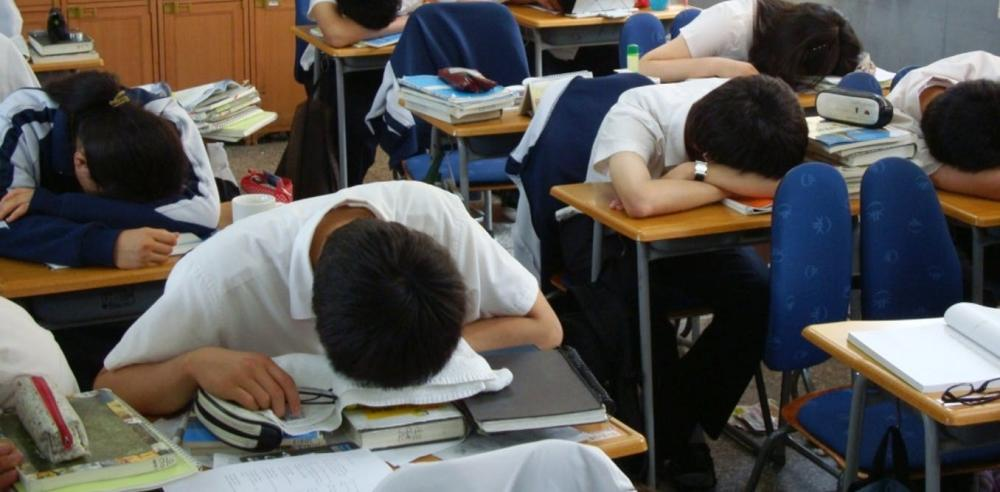
\includegraphics[height=5cm]{pausa.jpg}
    \end{center}
\end{frame}

\begin{frame}{Nerdminer}
    Nerdminer: 80K hashes per second
    \begin{center}
        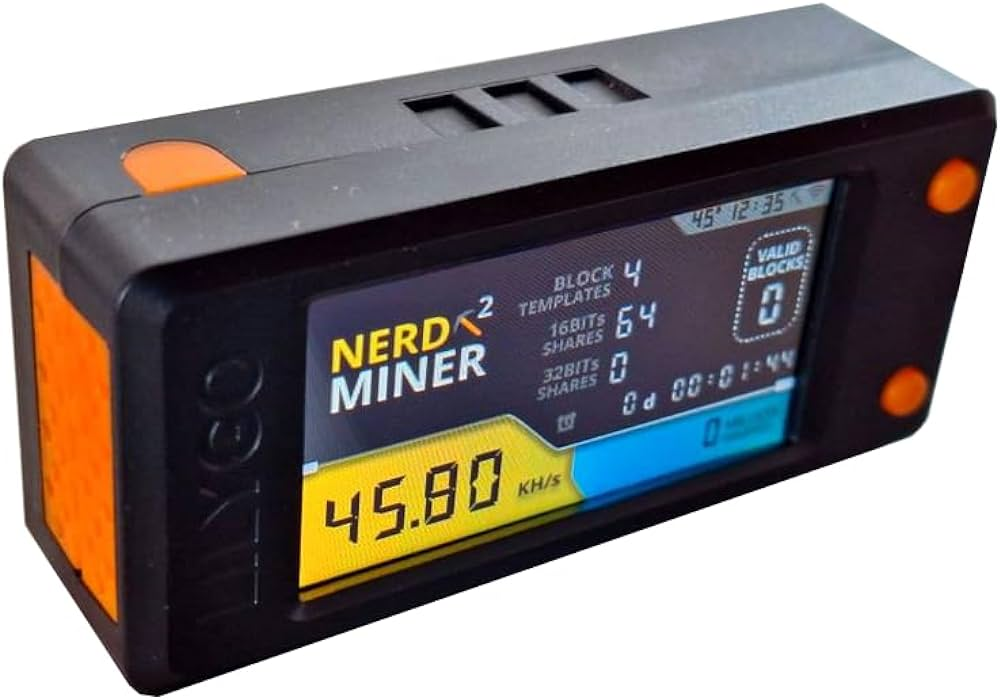
\includegraphics[height=5cm]{nerdminer.jpg}
    \end{center}
    \url{https://github.com/BitMaker-hub/NerdMiner_v2}
\end{frame}

\begin{frame}{Bitaxe}
    Bitaxe: 300G hashes per second
    \begin{center}
        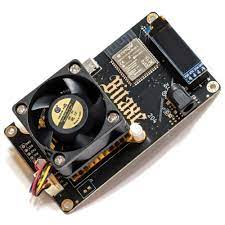
\includegraphics[height=5cm]{bitaxe.jpg}
    \end{center}
    \url{https://github.com/skot/bitaxe}
\end{frame}

\begin{frame}{Mining manuale}
    Mining Bitcoin with pencil and paper: 0.67 hashes per day
    \begin{center}
        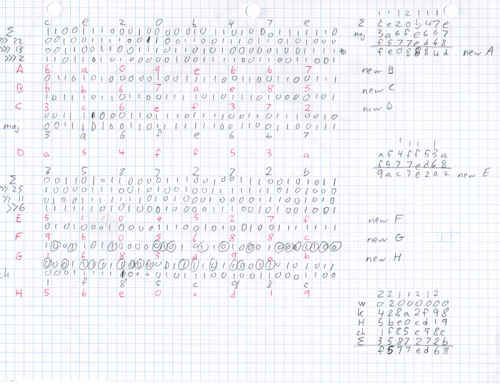
\includegraphics[height=5cm]{mining_manuale.png}
    \end{center}
    \url{https://www.righto.com/2014/09/mining-bitcoin-with-pencil-and-paper.html}
\end{frame}

\begin{frame}{Pool}
    \begin{center}
        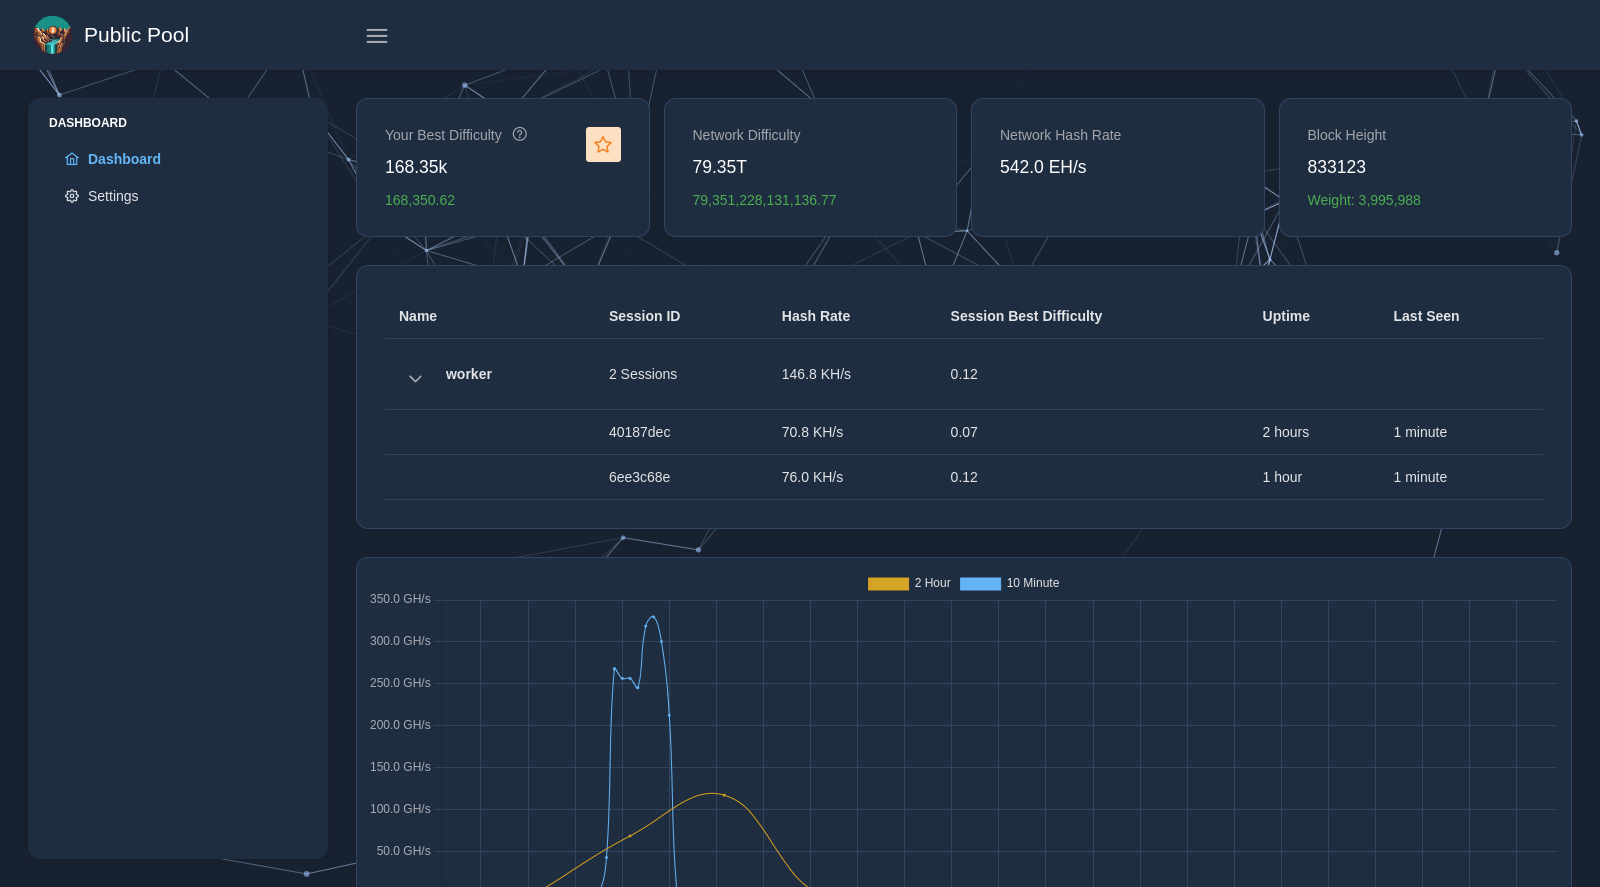
\includegraphics[height=5cm]{pool.png}
    \end{center}
    \url{https://web.public-pool.io/#/app/bc1q79qgpy5sc7n3fkmmc2920ycrhrt7e2fm6t7rw4}
\end{frame}

\section{Cambiando le Regole di Consenso}

\begin{frame}{Come cambiare le regole di consenso?}
Le regole del consenso determinano la validità delle transazioni e dei blocchi e possono essere modificate (mai retroattivamente) ma:
\begin{itemize}
    \item Le modifiche richiedono una forte convergenza di tutti gli attori
    \item Sono più semplici in caso di bug
    \item Le nuove funzionalità vengono testate per anni prima di essere consolidate
    \item La tendenza è quella di non cambiare più il protocollo (ossificazione)
    \item Possono generare hardfork ovvero lo split definitivo della catena
\end{itemize}
\end{frame}

\begin{frame}{Hardfork vs. softfork}
    \begin{center}
        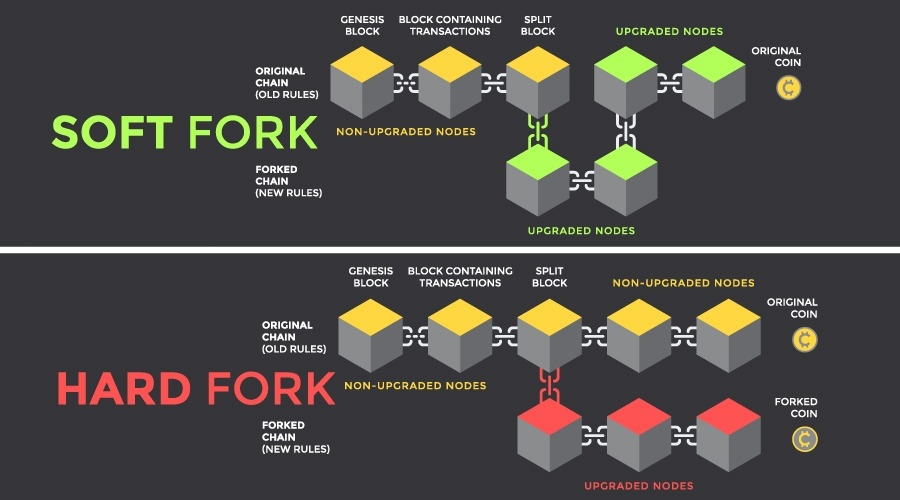
\includegraphics[height=5cm]{forks.jpg}
    \end{center}   
\end{frame}

\section{Attacchi al Consenso}

\begin{frame}{Perché avere il 51 per cento dell'hashing power è pericoloso?}
    Un attacco al cinquantun per cento si verifica quando un singolo miner o un gruppo di miner prende il controllo della maggioranza.

    \begin{center}
        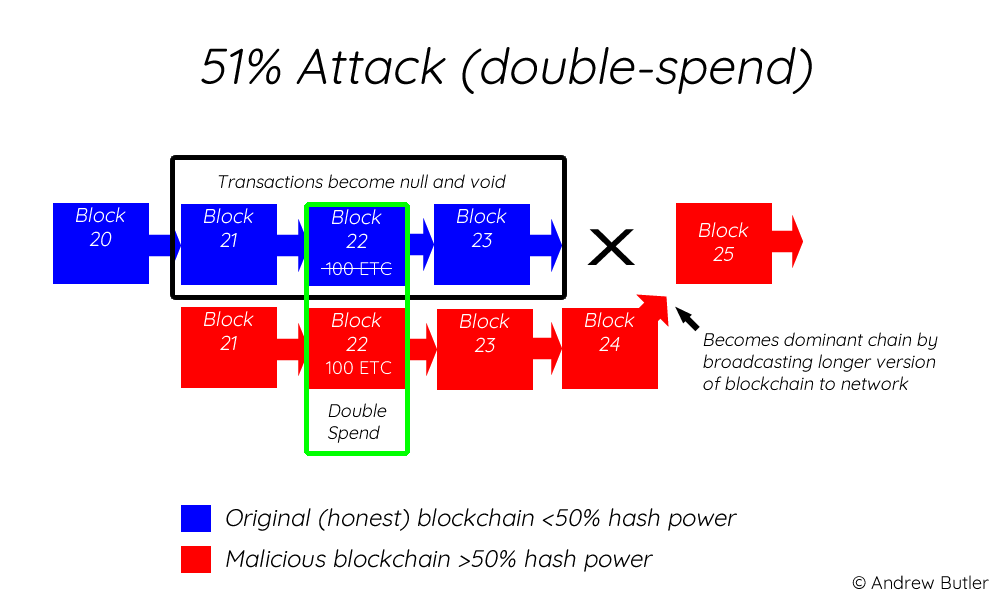
\includegraphics[height=5cm]{double_spend.png}
    \end{center}
\end{frame}

\begin{frame}{Se il problema sono le pool ...}
    Allora stratum v2 potrebbe risolverlo.

    Stratum v2 è un nuovo protocollo che sposta parte delle decisioni dalla pool ai singoli miner, un attacco controllando il cinquantun per cento dei singoli miner è più difficile.
\end{frame}

\section{Bibliografia}

\begin{frame}{Bibliografia} 
    \begin{itemize}
        \item Andreas M. Antonopoulos, "Mastering Bitcoin", 2015
        \item Adam Back, "Hashcash-a denial of service counter-measure", 2002
        \item Satoshi Nakamoto, "Bitcoin: A Peer-to-Peer Electronic Cash System", 2008
        \item Hal Finney, "Reusable Proofs of Work", 2004
    \end{itemize}
\end{frame}

\begin{frame}{Altre risorse} 
Tra le altre risorse utili mi piace citare:
    \begin{itemize}
        \item Ovviamente \href{https://t.me/BitPolimi}{BitPolimi} che ha organizzato queste lezioni.
        \item \href{http://satoshispritz.it}{Satoshi Spritz} - eventi serali a scadenze regolari per parlare di Bitcoin (a Milano ci incontriamo ogni mercoledì dalle 18).
        \item \href{https://t.me/ventunobtc}{Ventuno} - Podcast, raccolta di libri e materiali su Bitcoin.
        \item \href{http://officinebitcoin.it}{Officine Bitcoin} - lezioni su telegram da 30 minuti per la risoluzione di problemi pratici.
    \end{itemize}
\end{frame}


\begin{frame}{Domande} 
    \begin{center}
        
\includegraphics[height=5cm]{domande.jpg}
    \end{center}
\end{frame}

\begin{frame}[plain]
    \begin{center}
        
\includegraphics[height=8cm]{fine.jpg}
    \end{center}
\end{frame}

\end{document}
